% !TEX TS-program = pdflatex
% !TEX encoding = UTF-8 Unicode

% This is a simple template for a LaTeX document using the "article" class.
% See "book", "report", "letter" for other types of document.

\documentclass[11pt]{book} % use larger type; default would be 10pt

\usepackage[utf8]{inputenc} % set input encoding (not needed with XeLaTeX)

%%% PAGE DIMENSIONS
\usepackage{geometry}
\geometry{a4paper}
% \geometry{margin=2in} % for example, change the margins to 2 inches all round
% \geometry{landscape} % set up the page for landscape
%   read geometry.pdf for detailed page layout information

\usepackage{graphicx}
\graphicspath{{./images/}}
\usepackage[parfill]{parskip} % Activate to begin paragraphs with an empty line rather than an indent

%%% PACKAGES
\usepackage{booktabs} % for much better looking tables
\usepackage{array} % for better arrays (eg matrices) in maths
\usepackage{paralist} % very flexible & customizable lists (eg. enumerate/itemize, etc.)
\usepackage{verbatim} % adds environment for commenting out blocks of text & for better verbatim
\usepackage{subfig} % make it possible to include more than one captioned figure/table in a single float

%%% HEADERS & FOOTERS
\usepackage{fancyhdr} % This should be set AFTER setting up the page geometry
\pagestyle{fancy} % options: empty , plain , fancy
\renewcommand{\headrulewidth}{0pt} % customize the layout...
\lhead{}\chead{}\rhead{}
\lfoot{}\cfoot{\thepage}\rfoot{}

%%% BIBLIOGRAPHY
\usepackage{biblatex}
\addbibresource{sample.bib}

%%% CODE INSERTIONS
\usepackage{listings}
\renewcommand{\lstlistingname}{Code}
\usepackage{color}

\usepackage{hhline}
\usepackage{makecell}
\renewcommand\theadfont{\normalfont\bfseries}

%New colors defined below
\definecolor{codegreen}{rgb}{0,0.6,0}
\definecolor{codegray}{rgb}{0.5,0.5,0.5}
\definecolor{codepurple}{rgb}{0.58,0,0.82}
\definecolor{backcolour}{rgb}{0.95,0.95,0.92}

%Code listing style named "mystyle"
\lstdefinestyle{mystyle}{
  % backgroundcolor=\color{backcolour},   commentstyle=\color{codegreen},
  % keywordstyle=\color{magenta},
  % numberstyle=\tiny\color{codegray},
  % stringstyle=\color{codepurple},
  % basicstyle=\footnotesize,
  % breakatwhitespace=false,
  breaklines=true,
  captionpos=b,
  keepspaces=true,
  numbers=left,
  numbersep=5pt,
  showspaces=false,
  showstringspaces=false,
  showtabs=false,
  tabsize=2
}

%"mystyle" code listing set
\lstset{style=mystyle}

%%% SECTION TITLE APPEARANCE
\usepackage{sectsty}
\allsectionsfont{\sffamily\mdseries\upshape}

%%% ToC (table of contents) APPEARANCE
\usepackage[nottoc,notlof,notlot]{tocbibind} % Put the bibliography in the ToC
\usepackage[titles,subfigure]{tocloft} % Alter the style of the Table of Contents
\renewcommand{\cftsecfont}{\rmfamily\mdseries\upshape}
\renewcommand{\cftsecpagefont}{\rmfamily\mdseries\upshape} % No bold!

\title{Survival Analysis with Apache Spark and Apache SystemML on Stackexchange}
\author{Mateo Álvarez Calvo}
%\date{} % Activate to display a given date or no date (if empty),
         % otherwise the current date is printed

\newcolumntype{C}[1]{>{\centering\arraybackslash}m{#1}}   %% centered
\newcolumntype{R}[1]{>{\raggedleft\arraybackslash}m{#1}}  %% right aligned



\begin{document}

\maketitle

\newpage
\tableofcontents
\listoffigures
\listoftables
\lstlistoflistings


\chapter{Introduction \& main goals}
  \label{sec:introduction}
  Many studies have been done over the Stackexchange community [Mamykina, Manoim et al 2011], one of the biggest Q\&A sites in the world. The present is yet another study over the data of the famous site, but in this case, the study has two particularities, the use of Apache Spark with the library of Apache SystemML for the processing in a parallel environment, and the use of Survival Analysis to analyze the impact of the variables in the time an answer is accepted for each question, the "survival of each question" in the community.


  \section{Main technologies}

    As one of the biggest Q\&A communities, Stackexchange has large amount of data of each interaction.
    Stackexchange is separated in several communities, regarding different topics. These communities can be small, as \emph{DevOps} and \emph{InternetOfThings} or really big, as \emph{AskUbuntu} and \emph{Stackoverflow}, the main developers community. This particularity makes necessary the use of technologies prepared to process large amounts of data, in the later case.

    The purpose of the present study is to analyze a medium size community, so a distributed processing technology has to be used. For this purpose, Apache Spark, the latest distributed open-source processing technology, has been chosen to parallelize the operations on the data.

    Spark ML is the machine learning library of spark, which contains the ML algorithms. Although it includes some Survival Analysis algorithms, all of them are parametric models, which require to specify a hazard function shape in order to be used. This rests flexibility to the models, and for this study the hazard function is not known, so it is wise to start exploring the data with a non-parametric model, KM estimates, for example, and then apply some semi-parametric model, in this case Cox Proportional Hazards model. The absence of non or semi parametric models in Spark ML gives an excuse to use SystemML, a machine learning library developed by IBM and recently adopted as an Apache Foundation project, which has non, semi and parametric algorithms for survival analysis, and is compatible with distributed processing frameworks as Spark or Hadoop.

    Regarding the development environment, Jupyter Notebook provides a simple and flexible interface for this analysis, and can also be integrated with Spark, allowing the complete development in just one environment.

  \subsection{Survival Analysis}

    Survival Analysis is a group of ML models used to predict the time passed until the occurrence of an event. Is a method widely used, specially in the medical and pharmaceutical environments, where the prediction of time until an event is frequently used.

    In this case, the objective of using these techniques is to understand the behavior of the variables with the time and to predict when will a posted question be answered. This idea has multiple uses, such as optimizations of the questions themselves, hour of the day, tags added, reputation of the user... or using for example StackOverflow as technical support for problems with software instead of paying the provider's technical support service.

  \subsection{Apache Spark}

    Apache Spark is a distributed processing technology developed in Scala by Databricks that represents the next step of Apache Hadoop. It includes the best parts of it, such as the Hadoop File System, but under a complete new paradigm that allows operations different from the famous map-reduce, using RAM as storage for results rather than writing to disk, lazy and optimized execution of tasks, and special focus on Machine Learning and SQL-like language, to mention some of the main features.

    The use of a distributed processing framework is not strictly necessary in this case, as the community to be analyzed is not that big, but is a good starting point to check the use of SystemML and Spark to make later analysis on a bigger network.

  \subsection{Apache SystemML}

    Recently included in the Apache Foundation Incubating  program, Apache SystemML is a machine learning framework that works in different modes, on both distributed frameworks, Spark or Hadoop, or stand alone mode, written in Java.

    This framework provides a language to implement distributed, optimized algorithms ready for big data in a high-level language syntax, for Python and R. Additionally, the framework provides a set of commonly used algorithms already implemented with the sintaxis.

    System ML can be executed in a variety of distributed and non distributed modes, with it's standalone mode, and the integration with Hadoop, and Spark via SystemML context, which allows the interaction through Scala, Python and R.


  \section{The Stackexchange data}
  \label{subsec:data_structure}

    % \subsection{Stack Exchange}

    Stack Exchange is a network of Q\&A websites created in 2009 after the great success of \emph{Stack Overflow} in 2008, a Q\&A community website for computer programming.

    Every question and answer, an all the contents of the communities are licensed under a \emph{Creative Commons Attribution-ShareAlike 3.0 Unported}, so the knowledge is free to be shared with others.

    Each community covers a different topic, from physics to software, and is structured in a reputation award format, each user's question and answer can be voted positively or negatively. This feature allows the self administration of the communities, which makes posible the existence of the network, as it is so big that an administrator or moderator could not manage. Whenever moderation is needed, for example when there is an argument, there is a specific place on each community to solve these problems, the Meta section, where the users post settle the disputes to be solved by administrators of the site. The reputation system works as gamification, giving users privileges and functionalities when they earn experience points.

    All these communities generate large amounts of data that Stackexchange facilitates every once in a while for data scientists and people in general to download and analyze. The data is available in a torrent file and each package has about 35 - 40 GB of compressed information.

    This compressed file has data from different communities for a certain period of time. In this case, the analysis is done over the Scifi community, which is a median size community for science-fiction Q\&A.

    \subsection{Scifi community}

    Scifi is a community in Stack Exchange that focuses on science fiction and fantasy. This community was selected because it has a medium size which is perfect to test the mentioned technologies in a reasonable period of time. Selecting just the data from Scifi community from the big compressed file, it weights around 110 MB in a 7z compressed format. This allows the computation on a local machine for experimentation and then scale the problem to a bigger community such as \emph{Ask Ubuntu} or \emph{Stack Overflow} when the process is refined and it can be launched remotely in a cluster. The data is divided in 8 files, and has the same structure for every community:

    \begin{table}[!ht]
      \centering
      \begin{tabular}{|c|p{0.3\textwidth}|c|}
        \hline

        File & Description & Size \\ \hline
        Votes.xml & Voting results for each question and answer & 84,1 MB \\ \hline
        Tags.xml & Relational table for tags on each question & 169 KB \\ \hline
        Users.xml & Users on the net & 16,7 MB \\ \hline
        PostLinks.xml & links to posts & 1,5 MB \\ \hline
        Posts.xml & List of all questions & 137,3 MB \\ \hline
        PostHistory.xml & All interactions of each post & 268,6 MB \\ \hline
        Comments.xml & List of all comments of each post & 66,3 MB \\ \hline
        Badges.xml & All users' badges & 16,1 MB \\

        \hline
      \end{tabular}
      \caption{List of files from the compressed Scifi folder}
      \label{tab:list_of_files}
    \end{table}

    Further details about the relational database structure is explained below, the objective is to show the variables obtained from the dataset so that the later variable selection is understood.

    \subsection{Votes.xml}

      This file contains information about votes of the users to each question. The file has the following structure:

      \begin{table}[!ht]
        \centering
        \begin{tabular}{|c|c|p{0.3\textwidth}|}
          \hline
          Feature & Data type & Description \\ \hline
          Id & Integer & Unique vote identifier \\ \hline
          PostId & Integer & Foreign key that indicates the post that was voted \\ \hline
          VoteTypeId & Integer & Type of vote, 1 for Downvote and 2 for Upvote \\ \hline
          CreationDate & Timestamp YYYY-MM-DDTHH:MM:SS.dScSmS & Time of votation \\ \hline
        \end{tabular}
        \caption{Votes table}
        \label{tab:votes}
      \end{table}

\newpage

    \subsection{Tags.xml}

      This file contains all tags and the posts that contains them. The file has the following structure:

      \begin{table}[!ht]
        \centering
        \begin{tabular}{|c|c|p{0.3\textwidth}|}
          \hline

          Feature & Data type & Description \\ \hline
          Id & Integer & Unique tag identifier \\ \hline
          TagName & Text & Name of the tag \\ \hline
          Count & Integer & Number of times used \\ \hline
          ExcerptPostId & Integer & \\ \hline
          WikiPostId & Integer & \\

          \hline
        \end{tabular}
        \caption{Tags table}
        \label{tab:tags}
      \end{table}

    \subsection{Users.xml}

      This file contains information about users. The file has the following structure:

      \begin{table}[!ht]
        \begin{tabular}{|c|p{0.3\textwidth}|p{0.35\textwidth}|}
          \hline

          Feature & Data type & Description \\ \hline
          Id & Integer & Unique user identifier \\
          Reputation & Integer & Reputation level of the user \\ \hline
          CreationDate & Timestamp YYYY-MM-DDTHH:MM:SS.dScSmS & User creation date \\ \hline
          DisplayName & Text & Alias to display on question \\ \hline
          LastAccessDate & Timestamp YYYY-MM-DDTHH:MM:SS.dScSmS & Last login date \\ \hline
          WebsiteUrl & Text & Site where the user signed up to \\ \hline
          Location & Text & Location of the user \\ \hline
          AboutMe & Text & Information user provided \\ \hline
          Views & Integer & User views count \\ \hline
          UpVotes & Integer & User up votes count \\ \hline
          DownVotes & Integer & User down votes count \\ \hline
          AccountIf & Integer & Unique user identifier \\

          \hline
        \end{tabular}
        \caption{Users table}
        \label{tab:users}
      \end{table}

\newpage

    \subsection{PostLinks.xml}

      This file contains information about relation between posts. The file has the following structure:

      \begin{table}[!ht]
        \begin{tabular}{|c|p{0.3\textwidth}|p{0.35\textwidth}|}
          \hline

          Feature & Data type & Description \\ \hline
          Id & Integer & Unique post links identifier \\
          CreationDate & Timestamp YYYY-MM-DDTHH:MM:SS.dScSmS & Post links creation date \\ \hline
          PostId & Integer & Post unique identifier \\ \hline
          RelatedPostId & Integer & Unique identifier of the post related to the PostId \\ \hline
          LinkTypeId & Integer & Type of relation between posts \\

          \hline
        \end{tabular}
        \caption{Post links table}
        \label{tab:postlinks}
      \end{table}

    \subsection{Badges.xml}

      This file contains information about the badges the user has obtained.

      \begin{table}[!ht]
        \centering
        \begin{tabular}{|c|p{0.3\textwidth}|p{0.35\textwidth}|}
          \hline

          Feature & Data type & Description \\ \hline
          Id & Integer & Unique Badge identifier \\ \hline
          UserId & Integer & Unique identifier of the user who obtained the badge \\ \hline
          Name & Text & Name of the badge \\ \hline
          Date & Timestamp YYYY-MM-DDTHH:MM:SS.dScSmS & Time the user obtained the badge in extended format \\ \hline
          Class & Integer & Type of the badge \\ \hline
          TagBased & Boolean & Whether the badge is based on a tag or not \\

          \hline
        \end{tabular}
        \caption{Badges table}
        \label{tab:badges}
      \end{table}

\newpage

    \subsection{Posts.xml}

      This file contains all questions posted along with the accepted answers and other info related to the time and user who posted the question. The file has the following structure:

      \begin{table}[!ht]
        \centering
        \begin{tabular}{|c|p{0.3\textwidth}|p{0.35\textwidth}|}
          \hline

          Feature & Data type & Description \\ \hline
          Id & Integer & Unique question identifier \\ \hline
          PostTypeId & Integer & Type of post codified as integer \\ \hline
          CreationDate & Timestamp YYYY-MM-DDTHH:MM:SS.dScSmS & Time of question creation in extended format \\ \hline
          Score & Integer & Question's score, calculated from the users' votes \\ \hline
          ViewCount & Integer & Count of all visualizations of the question \\ \hline
          Body & Text & The question itself, in utf8 format \\ \hline
          OwnerUserId & Integer & Id of the user who posted the question \\ \hline
          LastEditorUserId & Integer & \\ \hline
          LastEditDate & Timestamp YYYY-MM-DDTHH:MM:SS.dScSmS & Last edition date \\ \hline
          LastActivityDate & Timestamp YYYY-MM-DDTHH:MM:SS.dScSmS & Last interaction with the question time \\ \hline
          Title & Text & Title of the question \\ \hline
          Tags & Text & Tags added to the question \\ \hline
          AnswerCount & Integer & Number of answers to the question \\ \hline
          CommentCount & Integer & Number of comments to the question posted \\ \hline
          FavoriteCount & Integer & Number of times the question has been added to favorite by another user \\ \hline
          ClosedDate & Timestamp YYYY-MM-DDTHH:MM:SS.dScSmS & Time the question has been closed \\ \hline
          CommunityOwnedDate & Timestamp YYYY-MM-DDTHH:MM:SS.dScSmS & Time \\

          \hline
        \end{tabular}
        \caption{Posts table}
        \label{tab:posts}
      \end{table}

\newpage

    \subsection{PostHistory.xml}

      This file contains information about the interactions with each post. The file has the following structure:

      \begin{table}[!ht]
        \centering
        \begin{tabular}{|c|p{0.3\textwidth}|p{0.35\textwidth}|}
          \hline

          Feature & Data type & Description \\ \hline
          Id & Integer & Unique interaction identifier \\ \hline
          PostHistoryTypeId & Integer & Type of interaction with the post () \\ \hline
          PostId & Integer & Unique identifier of the post this interaction is related to \\ \hline
          RevisionGUID & Text &  \\ \hline
          CreationDate & Timestamp YYYY-MM-DDTHH:MM:SS.dScSmS & Time of question creation in extended format \\ \hline
          UserId & Integer & Unique identifier of the user that created the interaction with the post \\ \hline
          Text & Text & Text the user introduced on the interaction \\ \hline

          \hline
        \end{tabular}
        \caption{Post history table}
        \label{tab:posthistory}
      \end{table}

    \subsection{Comments.xml}

      This file contains the comments posted for every question created. The file has the following structure:

      \begin{table}[!ht]
        \centering
        \begin{tabular}{|c|p{0.3\textwidth}|p{0.35\textwidth}|}
          \hline

          Feature & Data type & Description \\ \hline
          Id & Integer & Unique comment identifier \\ \hline
          PostId & Integer & Unique identifier of the post this comment is related to \\ \hline
          Score & Integer & Total score of the comment \\ \hline
          Text & Text & Comment text \\ \hline
          CreationDate & Timestamp YYYY-MM-DDTHH:MM:SS.dScSmS & Time of comment creation in extended format \\ \hline
          UserId & Integer & Unique identifier of the user who posted the comment \\

          \hline
        \end{tabular}
        \caption{Comments table}
        \label{tab:comments}
      \end{table}

\newpage

  \section{Main Objectives}

    The main objective of this study is to test the scalability and integration of the proposed technologies, Spark, SystemML and Jupyter Notebook in the usecase of Stack Exchange communities, so further data analysis can be performed. This main goal is divided in three major objectives:

    \begin{itemize}

      \item Use Spark to make the data cleaning and create a script for further research on the Stackexchange site.

      \item Verify SystemML integration with Spark for further research and scalability.

      \item Use SystemML survival analysis algorithms to analyze Stackexchange's data and obtain conclusions on the main variables affecting the time taken by the community to answer each question.

    \end{itemize}

\newpage

\chapter{Technologies}
  \label{sec:technologies}

  The downloaded data from Stackexchange for the analysis weights about 40 GB, which is enough amount to consider distributed processing. Going down to the distributed processing frameworks, Apache Spark was chosen.

  \section{Apache Spark}

    Apache Spark is a fast and general-purpose cluster computing framework, widely used for data processing. It provides high-level APIs in Java, Scala, Python and R, and an optimized engine that supports general execution graphs. It also supports a rich set of higher-level tools including Spark SQL, a SQL-like language prepared for both SQL and NoSQL databases, MLlib and SparkML for machine learning and pipelines, GraphX for graph processing, and Spark Streaming.

    This distributed data processing framework was initially developed at the University of California, Berkeley's AMPLab, and donated to the Apache Software Foundation in February 2014, the first release was on May 30th 2014.

    Apache Hadoop presented some limitations that Apache Spark tried to solve:

    \begin{itemize}
      \item It is difficult to write most of the algorithms in a MapReduce form.
      \item It is very slow to write each iteration to disk, which, for example makes difficult to use Hadoop to process streaming.
      \item Apache Hadoop's support for iterative jobs and Machine Learning restricts it's use for this task.
      \item Apache Hadoop's SQL tools doesn't work well on complex queries, sometimes it doesn't work at all and other times it is quite slow as it writes on HDD each iteration.
      \item Streaming functionality is not supported
    \end{itemize}

    Some solutions Apache Spark provides to these problems are:

    \begin{itemize}
      \item Lazy computation, Spark only executes a set of tasks when a result is required. This gives the opportunity to optimize jobs before executing them, even at physical level the queries to the data are optimized.
      \item In-memory data caching, Spark scans HDD only once to read the input data and then uses RAM as much as it can, which is faster than scanning disk on every step.
      \item Specific Machine Learning libraries, Spark ML and Spark MLlib, including numerous algorithms prepared to run in a distributed mode.
      \item Spark SQL provides structured (SQL-like) query language for structured and not structured data in SQL or Dataframe API. One of the advantages of this library is the unified access to datastores with the same language, it even provides SQL functionality with streaming data. Other interesting advantages are at an optimization level, using Dataframe API, Spark can optimize operations and queries to the database, using the \emph{Catalyst} optimizer.
      \item Spark Streaming library allows users to process streaming data using microbatches
    \end{itemize}

    \subsection{Apache Spark Structure}

      Spark has a master-slave architecture and supports various resource managers: standalone, Mesos and YARN. The resource manager will only be in charge of identify the resources. Independently of the resource manager chosen, the Apache Spark architecture doesn't change.

      The deployment of Spark has two variants, client and cluster mode. On the client mode, the Driver is launched on the machine the process has been invoked, and it can be inside or outside the cluster. On cluster mode, the cluster manager is assigned to control the Driver process, and the process itself will be launched inside the cluster. In case Mesos is the cluster manager, it will require an additional service.

      Focusing on the Spark cluster mode\footnote{The architecture for client mode is the same, but running all the programs and processes in the same machine.}, the architecture is as follows \footnote{As explained on the Official Spark documentation \cite{spark_documentation}}:

      All the Spark applications run on the cluster nodes as independent sets of processes, all coordinated by the main program, called \emph{driver program}, that coordinates all the others through the \emph{sparkContext}.

      The driver program deploys executor programs on the worker nodes of the cluster via a resource manager, already installed and running on the cluster, which provides the resources needed for the execution of the jobs. The driver first converts the user program into tasks and after that it schedules the tasks on the executors.

      The executor programs are in charge of running individual tasks in a given Spark job, all sent by the driver program through the sparkContext. They are launched at the beginning of a Spark application and typically run for the entire lifetime of an application. Once they have run the task they send the results to the driver. They also provide in-memory storage for RDDs that are cached by user programs through Block Manager.

      Spark driver program has to be in continuous contact with the executors, as it has to coordinate the workflow and the specific tasks for each executor and monitors the status of them. Moreover, when a result is required by the user, and it is not saved to a datastore, the result will go back to the driver program. The driver can run in an external machine of the cluster, but, as it has to be in continuous communication with the executor programs, it has to be running all the time the executors are calculating and it can not be disconnected to the cluster.

      More than one application can run in the same cluster, as long as there are enough resources. Each application gets its own executor processes and run tasks in multiple threads. This has the benefit of isolating applications from each other, on both the scheduling side (each driver schedules its own tasks) and executor side (tasks from different applications run in different JVMs), all of them running in different java processes, in general in different machines. However, it also means that data cannot be shared across different Spark applications (instances of SparkContext) without writing it to an external storage system.

      \begin{figure}[!ht]
        \centering
        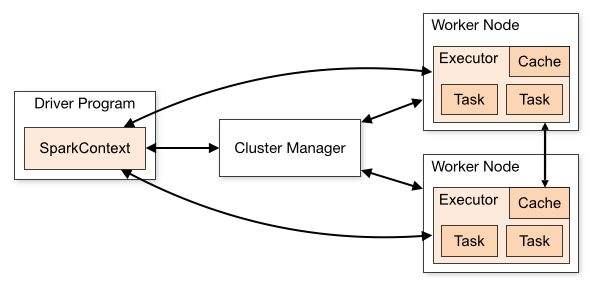
\includegraphics[width=\textwidth]{cluster-overview.png}
        \caption{Spark Cluster Mode Architecture, from \cite{spark_documentation}}
        \label{img:spark_architecture}
      \end{figure}

      Apache Spark is formed by the Spark Core API, available in R, SQL, Python, Scala and Java languages, and built up on it four main libraries: Spark SQL + DataFrames, Spark Streaming, Spark MLlib, Spark ML and GraphX, that complements functionality for Spark, specially on the parts Hadoop failed, Machine Learning, SQL and Streaming. There are other libraries but these are the essential.

      These libraries can be imported independently and combined to be used at the same time, for example, Spark SQL can be used in a Streaming environment with Spark Streaming library and this way SQL queries can be launched in

    \subsection{Apache Spark Data Structure}

      \subsubsection{RDDs}

        Apache Spark started with just one data structure, the RDDs. The RDD responds to Resilient Distributed Dataset, and have the following properties:

        \begin{itemize}
          \item Resilient: an RDD can be computed again in case of failure
          \item Distributed: the RDD can be partitioned and distributed over nodes, to parallelize the works
          \item Immutable: an RDD can not be modified, instead, a transformation is applied and other RDD is generated
          \item Lazy: RDDs represent a result of a series of operations and transformations over data, but it does not trigger any operation
          \item Statically typed: the values in the RDD are typed
        \end{itemize}

      \subsubsection{Dataframes}

        Dataframes are distributed collections structured in named columns, the idea is similar to the R dataframes. Dataframes are part of the Spark SQL API and are built up from RDDs, it is a higher level of data structure, which means that can take advantage of Catalyst to optimize the queries.

      \subsubsection{Datasets}

        Datasets are similar to dataframes, but also taking the static typing of the RDDs, combining the best of the two data structures.

        This static typing allows datasets to use Tungsten, Spark's optimized memory engine. Tungsten has direct access to off heap memory, to provide even better optimization, and uses data types to minimize the encoding and decoding of the data.

      \begin{figure}[!ht]
        \centering
        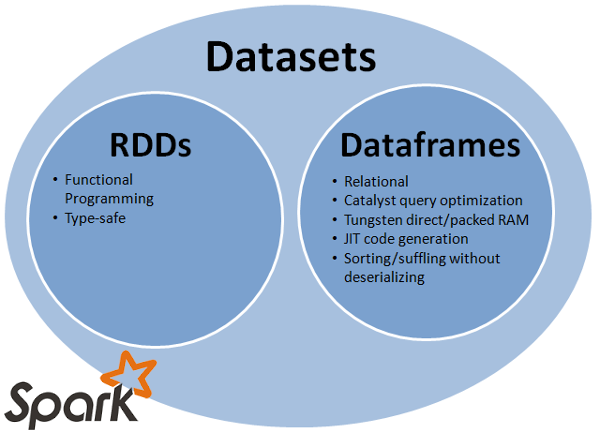
\includegraphics[width=0.75\textwidth]{RDD_dataframes_datasets_diagram.png}
        \caption{Differences between RDDs, dataframes and datasets, from \cite{RDD_dataframes_datasets_diagram_blog}}
        \label{img:RDD_dataframes_datasets_diagram}
      \end{figure}

      \subsubsection{Graphframes}

        Graphframes are structures used for graph storage and operations. Graphframes are composed by two dataframes, the first one contains all the vertices and the second one contains all the edges. This is useful as dataframes can be optimized by Catalyst. GraphFrames are not part of the Apache Spark core API, as there is still development to do.

      \subsubsection{Discretized Streams}
        Discretized Streams, or DStreams, are the basic data structure that Spark Streaming module uses for processing. This DStreams are essentially RDDs in time periods, and represent the data available on each time window. As Spark Streaming works with microbatches, small (or not so small) time intervals of data processing. For a time period, a DStream is basically an RDD, on which operations can be performed giving as a result another temporary RDD or DStream.

      \begin{figure}[!ht]
        \centering
        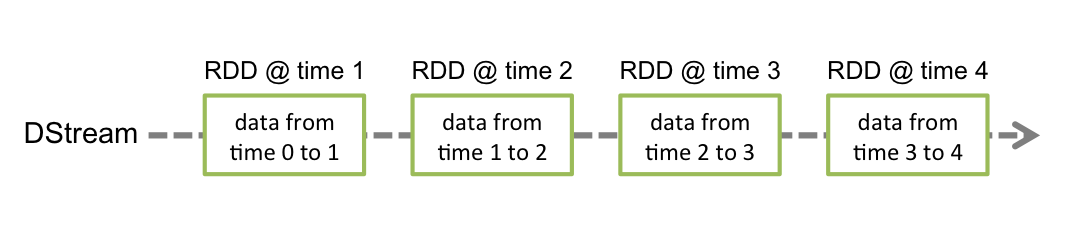
\includegraphics[width=0.75\textwidth]{streaming-dstream.png}
        \caption{DStream structure, from \cite{spark_documentation}}
        \label{img:DStream_squema}
      \end{figure}

      \subsubsection{Catalyst and Tungsten}

        As mentioned before, Spark has some specific tools to optimize the workflow when using dataframes and datasets, these optimizers focus both on I/O, writing and reading data, with Catalyst, and on the execution engine itself.

        Catalyst is the query optimizer, included in the Spark SQL API. As the execution is not done until an action is called, for example a calculation of a result, Spark can analyze the code and choose the order of operations, which means that, for example, when querying to a database to apply filters, those filters can sometimes, if the database is relational, be applied natively in the database, moreover the sequence of subsequent filters is analyzed in order to reduce the I/O on the database, which can lead to a significant reduction of time and resources, as usually the data available is abundant, but the data used for a process is significantly less. Catalyst works in four phases:

        \begin{itemize}
          \item The \emph{analysis phase} returns a logical plan where all the metadata from the data involved in the operation is known
          \item The \emph{logical optimization phase} consists on the optimization of the operations performed over the data using ruled-based optimizations
          \item The \emph{physical planning phase} uses cost-based models to select the best execution plan from the ones available after the logical optimization phase
          \item The \emph{code generation phase} is the final phase, where Spark compiles parts of the query code to Java bytecode, this speeds up the process as there is no need to use the Scala compiler at runtime to generate bytecode.
        \end{itemize}

        Tungsten is the execution engine's optimizer has been developed due to the improvement in the I/O operations thanks to Catalyst, and is focused on the performance of the CPU and the memory, it is focused on three major fields:

        \begin{itemize}
          \item Memory Management and Binary processing: java uses objects, which have a large memory overhead, increasing the size of space occupied to store more simple variables. Apart from Java objects, JVM uses Java Garbage Collector, which manages object creation and destruction according to the life cycle of each object. This is a complex task, as the life cycle can not always be estimated precisely, which causes overhead on the memory, keeping short life cycle objects when they are not necessary and viceversa. Spark understands the data flow through the stages of computation, so it is posible to have a better optimizer than the JVM, for that purpose, Spark introduces an explicit memory manager that converts most operations to use binary data rather than using Java objects and Garbage Collector.
          \item Cache-aware computation: when computing large amounts of data on an in-memory processing framework, not all data is able to fit in the machine's memory, so information is written to disk. This and fetching data from the main memory are time consuming operations, so large fractions of CPU time are spent on gathering data to process. The solution Spark provides to avoid spending so much time waiting for data to travel from disk or main memory is to design "cache-friendly algorithms" that uses L1/L2/L3 CPU cache as they are orders of magnitude faster than main memory.
          \item Code generation: Spark dynamically generates bytecode to evaluate expressions, such as SQL expressions rather than using an intermediate interpreter. Using some specific data structures such as dataframes, built from RDDs is an advantage, as data types are already known and specific code can be generate to treat the serialization as there are more information available.
        \end{itemize}


      \subsection{Spark Main APIs}

        \subsubsection{Spark Core API}

          The core API represents the basic structure of Spark, it can be addressed from any of the supported languages, scala, python, R and java. This API has the main functionality of Spark, which includes a set of operations, that includes Map-Reduce, but is not limited to them, as Hadoop is.
          Regarding the data management, This API contains the RDDs, explained above and the basic operations.[][][]

        \subsubsection{Spark SQL + DataFrames}

          The SQL layer over data is known as Spark SQL. It allows users to use a SQL-like language in Spark programs, to query both structured and not structured databases (SQL \& NoSQL), such as Postgres or MongoDB.

          The Spark SQL library also provides a main functionality in Spark that is gaining more importance over the time, the Dataframes.

          A Dataframe is a data structure introduced in the R programming language that has extended to the Data Science world as one of the most easy to use data structures. Dataframes in Spark are the same concept that in a non-distributed processing framework, but the implementation, as it is for a distributed environment is different, it is built from RDDs with a specific structure.

        \subsubsection{Spark MLlib + Spark ML}

          Spark has two main Machine Learning libraries, the first one, Spark MLlib, which is the basic library, that includes the main algorithms and is addressed with RDDs, the second one, Spark ML, which uses Spark MLlib but through DataFrames, and includes further functionality, such as Pipelines, a set of operations performed over data, that allows the user to build sequences of actions over Data Frames.

        \subsection{Spark Streaming}

          Spark Streaming is the real-time, streaming processing library of Spark. Unlike other streaming processing frameworks such as Apache Flink, Spark Streaming works with microbatches, remaining almost the same structure as Spark itself. The reason is to have the workers processing in time periods, this way the fault tolerance is more robust, as for each microbatch all the operations will be parallelized, and in case any worker falls down, the others complete the work. This way the latency is sacrificed in favor of robustness of fault tolerance.

          Spark Streaming runs on top of Spark, so that the benefits of the distribution, scalability and fault-tolerance are inherited from it, but it also has the advantage of using a similar sintaxis and the interoperability with other Spark libraries such as Spark-SQL, giving the possibility to process information with dataframes, with all the advantages they provide.

          Spark Streaming has support for numerous data stream sources, including Apache Kafka, ZeroMQ, TCP Socket or Flume, among others, this gives flexibility to the framework to connect to different applications.

          The workflow in Spark Streaming is the following: data enters at unspecified rate, it can be a specific amount every second or not a constant quantity, Spark Streaming will be in charge of distributing the data along the workers. Data is transformed into DStreams and distributed at a low level into RDDs, using the Spark Core functionalities, processed, and then returned to the microbatch. At the end of the microbatch, the application will return the processed data in DStreams. The schema below is a diagram of the explained workflow.

          \begin{figure}[!ht]
            \centering
            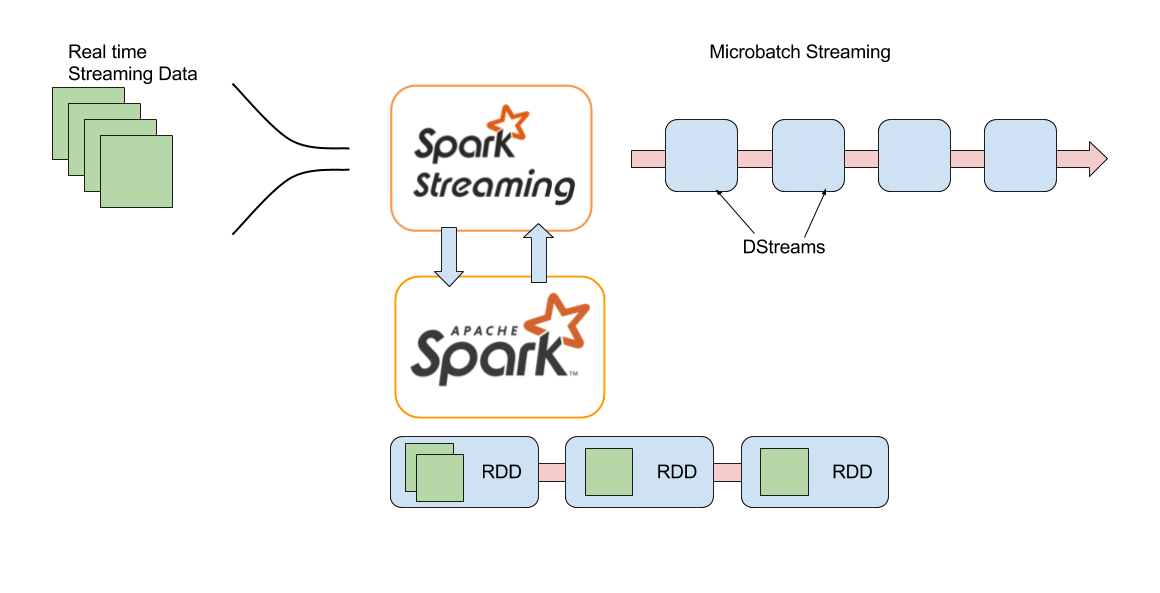
\includegraphics[width=0.75\textwidth]{Spark_Streaming_architecture.png}
            \caption{Spark Streaming workflow}
            \label{img:spark_streaming_workflow}
          \end{figure}


        \subsubsection{Spark GraphX}

          GraphX is Spark's graph library, which extends Spark's core API with special functionality for graphs. As commented before, Spark GraphX uses a different data structure, \emph{Graph}, a structure that provides functionality to introduce both vertices and edges for the graph. As all other libraries, the GraphX functionality can be mixed with all the rest of the framework, giving this library high flexibility.

          Unlike other Spark main libraries, GraphX does not provide access with other language than Scala, it can not be addressed with R nor Python, but it provides an increasing amount of distributed algorithms for graph analysis.

      \subsection{Spark workflow}

        There are three main phases on the execution of a program in Spark: definition of a DAG from the user's code, translation of the DAG to an execution physical plan, and scheduling and executing the plan in the cluster.

        \subsubsection{Definition of a DAG}

          The program defined by the user is a result of a series of operations (transformations and actions) done to a series of RDDs, the first RDD may be the ingest of the data, and the last one, the result the user wants to calculate. This series of operations over RDDs form a graph, an ordered sequence that leads to the final result, therefore the graph is directed, from the first RDD and operation to the last one, and is acyclic, it has a beginning and an end. This DAG is the logical representation of the execution of operations over RDDs and their partitions.

          On a lower level, the RDDs are the ones that contain the logical plan under the DAG, each RDD has one or more pointers to one or more parents, along with metadata about the relationship they maintain. These pointers allow an RDD to be obtained through it's ancestors, for example to be recalculated in case of a node failure.

        \subsubsection{Creation of physical plan}

          When executing, the DAG is translated to a physical plan which merges multiple operations into tasks. This execution is called whenever an action is called, this execution takes the DAG, looks to the latest RDD and goes backwards to the first ancestor to construct the operations needed. The output of this process is a \emph{job}, composed by a number of \emph{stages}, whose number depend on the operations performed over the RDDs, and \emph{tasks} in every stage.

          Formally, a task is a unit of execution that runs on a single machine, tasks group to form stages, which represent the operations performed over a partitioned data in a parallelized way, namely a stage is a group of tasks that will perform the same operation over a partitioned data.

          The number of stages created depend on the number of repartitions done to the data to obtain the final RDD, every time a shuffle operation is done to repartition the data over the machines, a new stage is created, for this reason, there can be less stages than group of parallelized tasks.

          \begin{figure}[!ht]
            \centering
            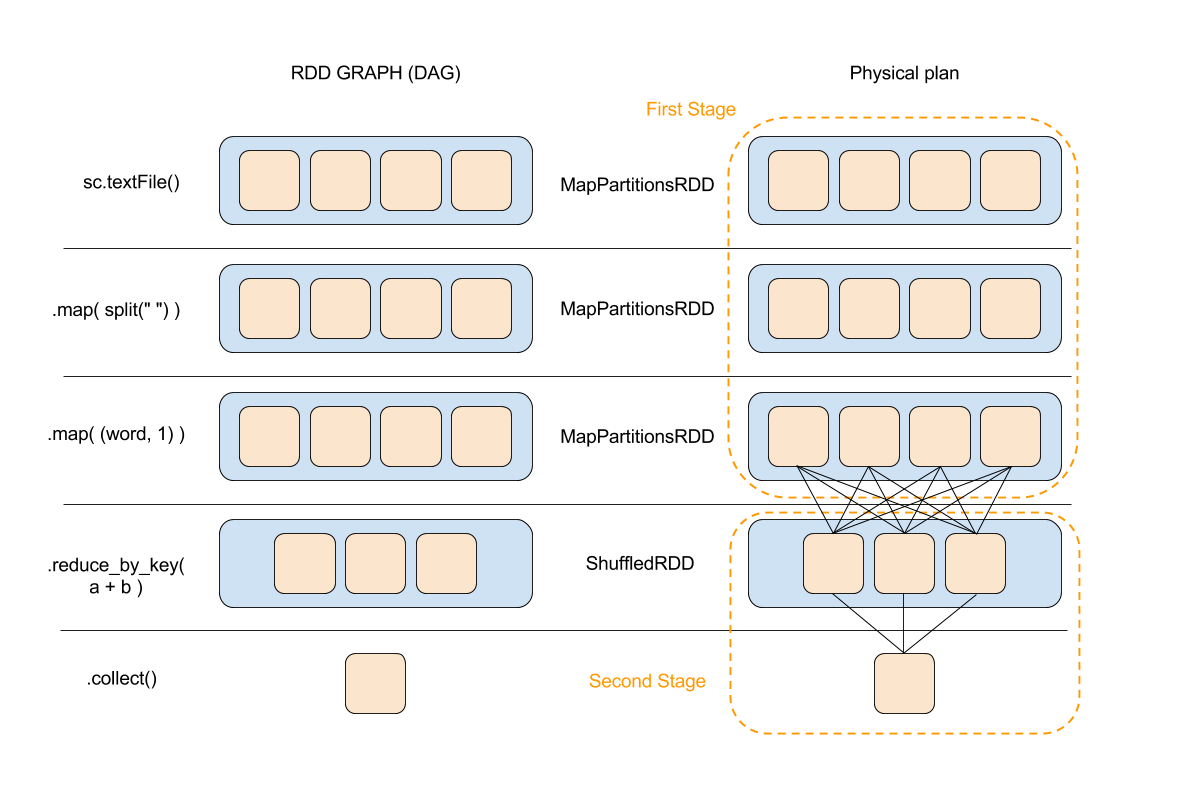
\includegraphics[width=0.8\textwidth]{DAG_to_phisical_plan.png}
            \caption{Example of translation of DAG to physical plan, for a word count application}
            \label{img:DAG_to_physical}
          \end{figure}

          It is interesting to note that, when using Spark SQL, the physical plan will be an optimized DAG, as shown before, using Tungsten and Catalyst.

          \begin{figure}[!ht]
            \centering
            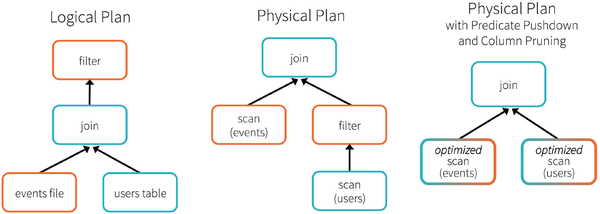
\includegraphics[width=0.8\textwidth]{spark_logical_to_phisical_plan.jpg}
            \caption{Example of an optimized physical plan from a DAG, using Spark SQL, from \cite{optimized_dag_to_physical}}
          \end{figure}

        \subsubsection{Scheduling and executing the physical plan on the cluster}

          Finally, the stages are executed in order, launching the tasks over the available nodes to compute the resulting RDD. As the execution runs in-memory, whenever a task fails, the entire sequence of operations of the stage has to be computed for the particular lost partition, but not all the tasks for all partitions. For this reason it is common to \emph{cache} the RDDs after a series of operations, avoiding this way to recalculate all the previous steps.

      \subsection{Spark UI}

        As seen in the sections above, there is a lot of information of the running process of a Spark application. To help the users monitor the application, configuration and the status of the cluster, Spark has a web user interface, in which all the information, the DAG, the physical plans, the storage with the cached data, the environment variables, the executors available and the SQL options.

        \begin{figure}[!ht]
          \centering
          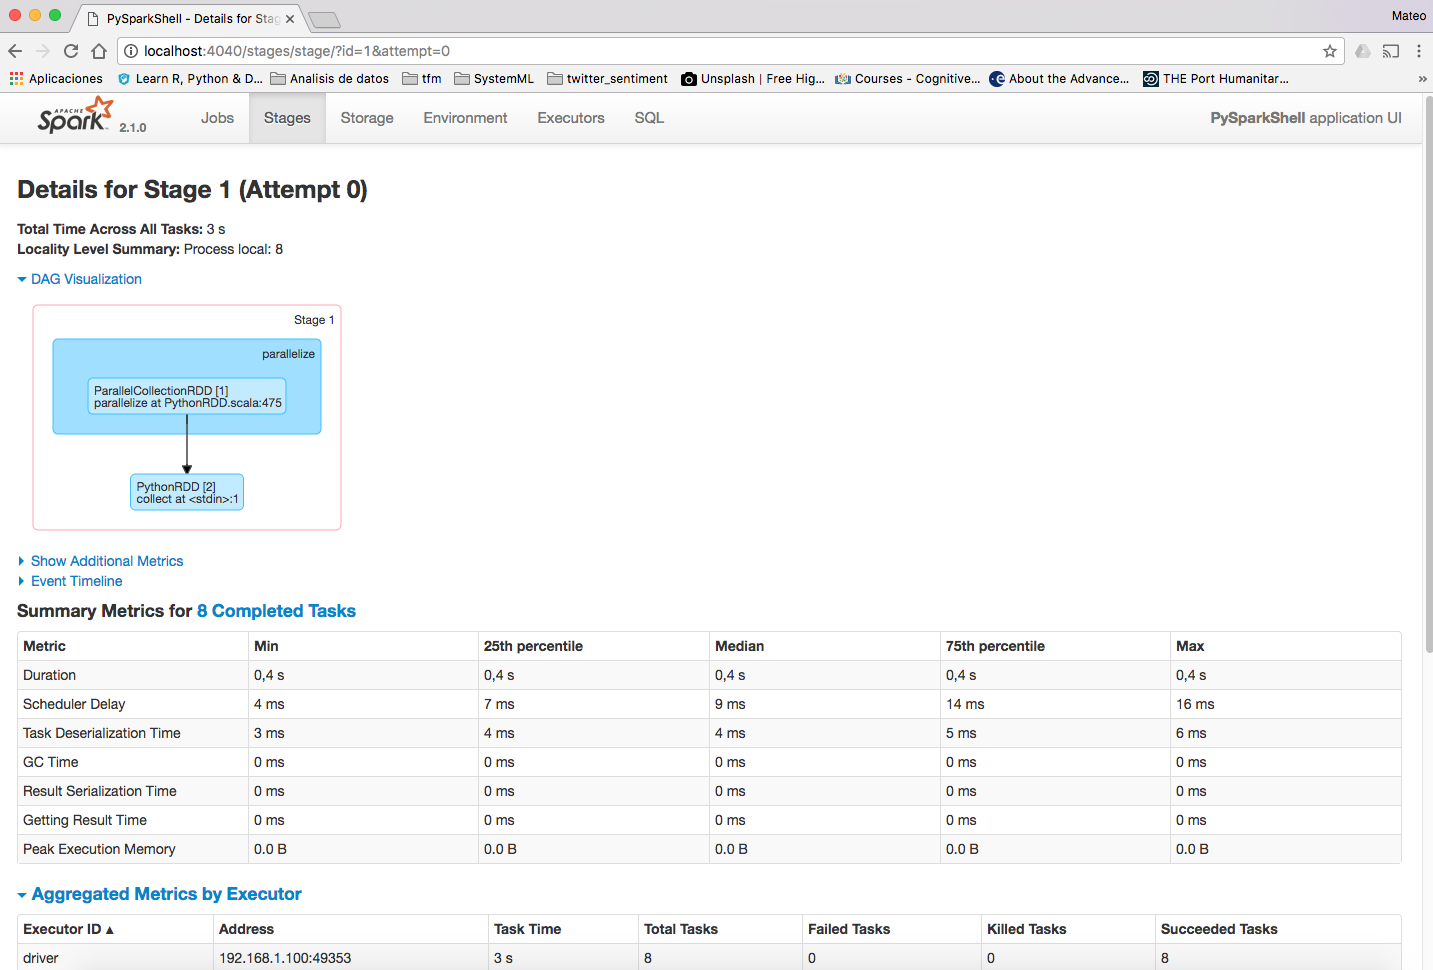
\includegraphics[width=0.8\textwidth]{spark_ui.png}
          \caption{Example of Spark UI}
          \label{img:spark_ui}
        \end{figure}

\newpage

  \section{Apache SystemML}

    Developed by IBM, SystemML started in 2007 as multiple projects involving machine learning with Hadoop, which in 2009 resulted in a single team dedicated to scalable machine learning research. Through 2009 and 2010, the team observed how clients developed machine learning algorithms, the workflow was (and still is) the following:

    First, a data scientist, working in a single PC, and developing in R or Python, used small amount of data to create a ML algorithm, this part of the process works fine, as the algorithms use small data, and the researchers can iterate fast to refine the algorithms. When the algorithm is ready, the data scientist gives it to a systems programmer who implements the algorithm in an optimized way with low level APIs, usually with a distributed processing framework, such as Spark or Hadoop. When the implementation is ready, the distributed algorithm is tested with big data and then the results return to the data scientist to verify the correct implementation of the distributed algorithm.

    The later part of the process leads to two major problems, the first one is the time spent for each iteration, which can be large, depending on the complexity of the process itself, and the second one is that during the reimplementation of the algorithm in the distributed framework, mistakes can be made, which leads to different results in big and small data, and to the depuration of the distributed code, a time consuming process.

    The objective of Apache SystemML is to attack these two problems, providing the data scientist with a interface in a Python or R like language that optimizes the code to run in a distributed environment, this way, the exact same code is executed in small and big data and the data scientist can verify the behavior of the algorithm on both contexts. The optimization of the code is done by translating this high-level language code written in R or Python to a scalable executable that can run on Spark (or Hadoop), with SystemML compiler and runtime.

    The project went open source on 2015 and entered Apache incubation in November 2015, with the first open-source binary release announced on January 2016. The latest release is from April 19$^{th}$ 2017, with the version \emph{v0.14.0-incubating-rc4}.

    \begin{figure}[!ht]
      \centering
      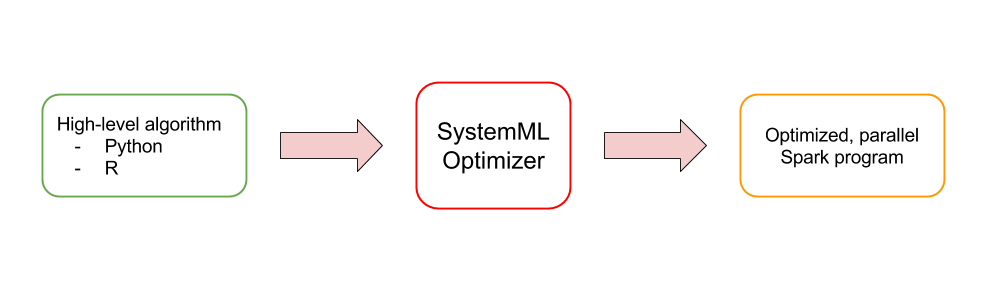
\includegraphics[width=\textwidth]{systemml_objective.png}
      \caption{Apache SystemML workflow}
      \label{img:systemml_workflow}
    \end{figure}

    \subsection{SystemML Architecture}

      Apache SystemML's architecture involves optimizers that converts code from the high level programming languages to specific code for Spark or Hadoop, for using a distributed infrastructure, or optimized single-node code, when the resources of one machine are enough for the process. All of this is done through three different stages, each one composed by different steps:

      \begin{figure}[!ht]
        \centering
        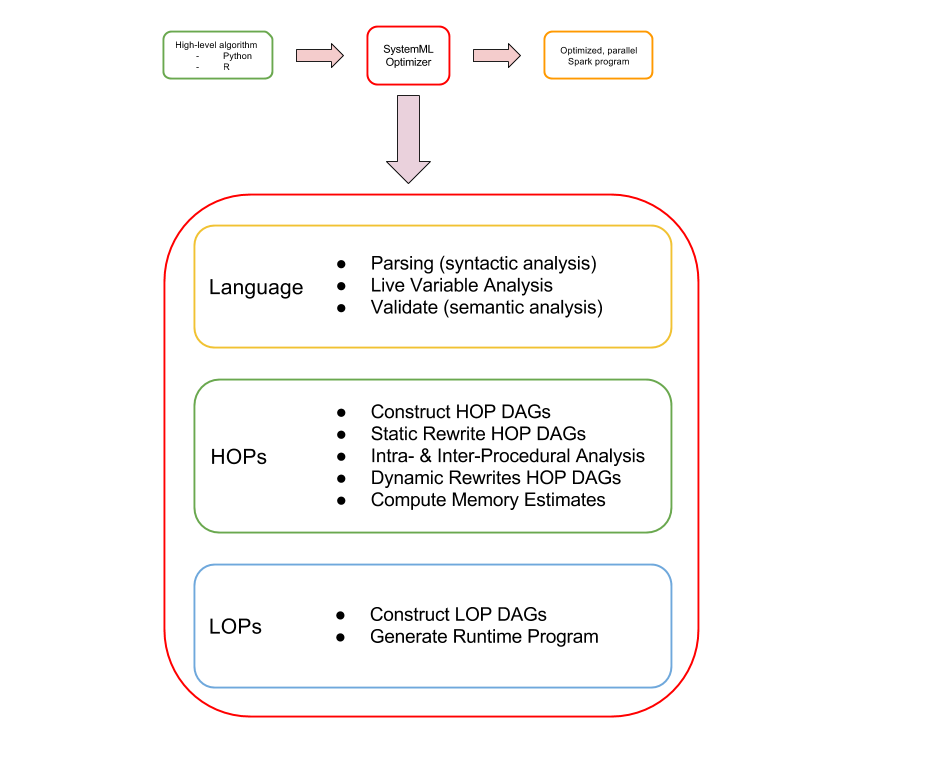
\includegraphics[width=\textwidth]{systemml_structure.png}
        \caption{SystemML Architecture}
        \label{img:systemml_architecture}
      \end{figure}

      \subsubsection{Language level}

        The first part is the \emph{language processor}, this piece is in charge of interpret the code written on R and Python and optimize the execution, converting complex and resource consuming operations to more optimized code. This piece is divided in three steps:

        The first step is to convert each operation into a hierarchical representation of statement blocks and statements, which means that the code written by the user is processed and understood by the optimizer, in order to be able to identify the resource and time consuming operations. This step analyzes the code not only lexically and syntactically, but also the order of operations and other basic aspects. The output of this step is the input code translated into the specific DML grammar.

        Once the operations are translated into the DML grammar, variables involved are analyzed, regarding, for example the input and output variables, their size in memory, and the data flow.

        The last step of the language level is to verify the correctness of the code obtained, checking dimensions of variables, necessary variables and parameters for operations among other things. This process is done over the whole program and validates expressions and code blocks, but also simulates the code execution in order to evaluate the resources necessary, analyzing the conditionals and loops, given that the optimizer already knows the size of the variables, as it has been checked on the first step.

      \subsubsection{Hight-level Operators (HOPs)}

        This phase of the optimization consists on structuring the operations in order to be able to rewrite the code in a more optimized way, for example changing the order of operations when it implies less resource consumption. To do so, from each basic block of statements, a high-level operators DAG is created, where the nodes represent operations and their outputs, and edges represent data dependencies between operations.

        As a result of this process, a single operator tree is built with all the statements and operators of the code. This tree represents a data flow graph is then used to build HOP DAG rewrites. These rewrites are size-independent transformations, for example format conversions or algebraic simplifications.

        After this rewrite phase, a simulation of the size of the variables and operations is performed, this way, the program is able to estimate if the execution of all the code is posible or adequated in one machine, otherwise it will be distributed over the machines available.

        The fourth step of this phase is to apply dynamic HOP DAG rewrites, this rewrites comprise simplifications done over the operations when the size is enough and cost-based rewrites, for example, the order of operations in matrix algebra, or the transposition of some matrixes over others depending on the size of them.

      \subsubsection{Low-level Operators (LOPs)}

        The last part of the optimizer focuses on low-level operations, generating again DAGs, representing operations in the nodes and data dependencies on the edges. These operations are optimized at a physical level, taking into account the specific backend and resources available in which the program will run, focusing specially on MR, instructions run in a Map-Reduce paradigm and CP (Control Program), operations executed in-memory.

        At the end of this phase, the main program is compiled and executables are generated for the specific backend used, wether it is in a distributed or a single node execution.

      \subsubsection{Runtime-Level}

        Apart from the work done by the optimizer in the stages previous to the execution of the code, it will also be available during the execution of the program. This way, the optimizer can analyze the real time execution and re-compile parts of the code. This is specially important when the execution is in a distributed environment and the optimizer have not had access to the data sizes, which will be available during runtime, giving the opportunity to make live changes and re-compilations of the code.

      The use of the optimizer does add an overhead to the execution of the program, typically around $200ms$ per script on the language-level, about $10ms$ per DAG on the HOP-level and $<1ms$ on the recompilation, including LOP-level.

    \subsection{SystemML Algorithms}

      Apart from its general purpose big data analysis capabilities, SystemML has a quite estense algorithm catalog, algorithms that are implemented over the optimizers and thus distributable whenever it is more efficient. Among the catalog SystemML provides, there is an interesting section, specially for this study, the Survival Analysis algorithms, this catalog includes a non-parametric model, the \emph{Kaplan-Meier Estimates model}, and one of the most famous semi-parametric model, the \emph{Cox Proportional Hazards model}. As it'll be explained later, the non-parametric algorithms are useful for exploratory analysis over the data, to have a first approach to the problem, while semi-parametric, and parametric, algorithms are used for further research over the data, giving much more information on the effect of the variables over the survival time.

      The main advantage of the semi-parametric models over the parametric models is that the former need less information of the problem itself, not requiring to provide a hazard shape beforehand, while the latter require some assumptions on the behavior of the hazard function on the problem. As it will be shown, this is an important advantage, as when dealing with an unexplored field, the hazard function is not usually known, having the semi-parametric models the advantage of being more flexible.

      Apache Spark's MlLib also has survival analysis algorithm, in particular, the \emph{Survival Regression with Accelerated Failure Time (AFT)} algorithm, a parametric algorithm easier to parallelize than the Cox Proportional Hazards model. This implementation of the AFT is similar to the one implemented on R, but in a distributed way, and uses a \emph{Weibull} distribution function as the hazard function shape. This is one of the main reasons SystemML was chosen for this study, as, unlike Spark, it has a non-parametric algorithm for exploratory analysis of the problem and a flexible semi-parametric algorithm, which is ideal for this study, as the shape of the hazard function is unknown.

  \section{Reproducible research with Python, Scala and Jupyter}

    Regarding the selection of the development environment, it was important to use a standardized one so that the analysis could be reproduced by anyone. Jupyter notebook is one of the most commonly used, specially in the education and investigation institutions. It is easy to use and configure, and flexible, as different kernels (code interpreters) can be configured, even for the same language with different set of libraries. It can be easily integrated with Big Data technologies, such as databases or Spark itself, and it does not have appreciable effect over the performance of the execution of code.

    Jupyter Notebook is an open-source web application that contains code interpreters and other functionalities that allow users to develop code and write and share documents. It works with a dedicated file type, the .ipynb, notebooks on which the user can write both code and text in a cell distribution, cells that can be executed independently, having, as a result, an interactive shell for the selected code interpreter. It has interactive interpreters for many languages, including python, ruby, scala, R, etc, as well as markdown interpreters.

    \begin{figure}[!ht]
      \centering
      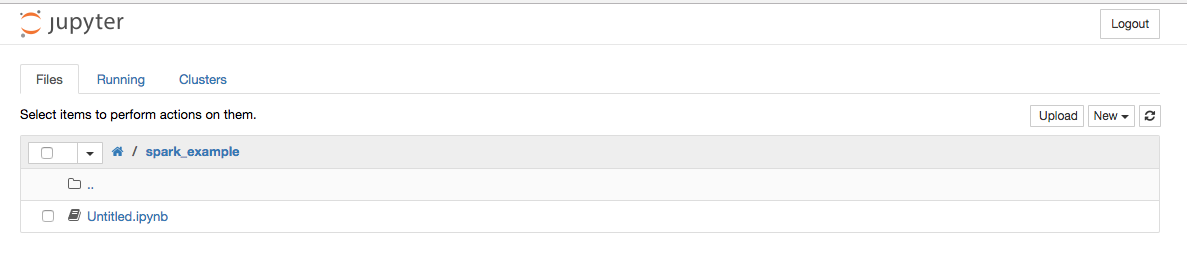
\includegraphics[width=\textwidth]{jupyter_notebook.png}
      \caption{Jupyter Notebook environment example}
      \label{jupyter_notebook_environment}
    \end{figure}

    Another important advantage of Jupyter Notebook is its simple integration with Spark, it can be launched directly from python via \emph{findspark} library, launching an embebed interactive Spark Shell, to execute the Spark code directly from the cells of the notebook, or it can be configured to be the launched when the Spark Shell is executed.

    \begin{figure}[!ht]
      \centering
      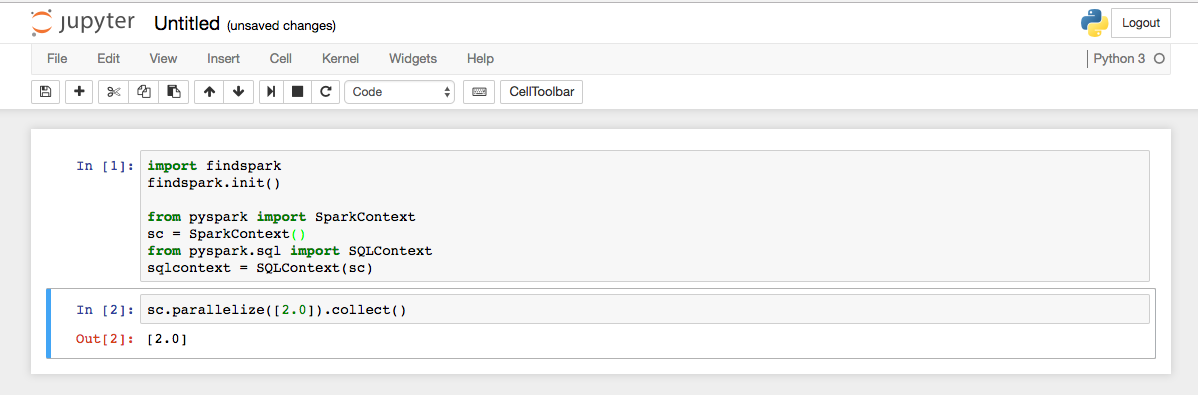
\includegraphics[width=\textwidth]{spark_notebook_example.png}
      \caption{Example of a python3 notebook with Spark integrated, running in standalone mode}
      \label{notebook_spark_example}
    \end{figure}

    To configure the same environment as the one used in this study, some steps have to be followed:

    \subsection{Environment setup}

      The versions of the software used for this study are listed below:

    \begin{table}[!ht]
      \centering
      \begin{tabular}{| c | c |}
        \hline

        Technology & Version \\ \hline
        Jupyter Notebook & 4.3.1 \\ \hline
        Python & 3.5 \\ \hline
        Scala & 2.11 \\ \hline
        Toree kernel & 0.2.0.dev1 \\ \hline
        Spark & 2.1 \\ \hline
        SystemML & 0.12.0 \\

        \hline
      \end{tabular}
      \caption{Technologies and versions used}
    \end{table}

    The first step is to setup Jupyter Notebook, either running it in a Docker container or installing it directly on the machine. The docker image can be obtained entering the following command in a shell: \emph{docker pull jupyter/notebook}. Regarding the other option, installing it, the instructions can be found in the following link:

    \emph{http://jupyter.readthedocs.io/en/latest/install.html}.

    Once Jupyter Notebook is running, the kernels have to be configured. In this study, Scala and Python were used for the data processing, so both kernels were configured. The python kernel is usually configured, as it comes with the IPython kernel installation, if not, follow the guide[][][][][]. To install the scala kernel, several options can be considered, as there are several implementations of the scala kernel. The chosen one was Scala Toree.

    Apart from the kernels, some dependencies must be installed to do the data processing in python, those dependencies are:

    \begin{itemize}
      \item appnope==0.1.0
      \item bokeh==0.12.4
      \item botocore==1.5.43
      \item findspark==1.1.0
      \item ipykernel==4.5.2
      \item ipython==5.3.0
      \item ipython-genutils==0.1.0
      \item matplotlib==2.0.0
      \item notebook==4.3.1
      \item numpy==1.12.0
      \item pandas==0.19.2
      \item py4j==0.10.4
      \item pyparsing==2.2.0
      \item python-dateutil==2.6.0
      \item scipy==0.18.1
      \item systemml==0.14.0
      \item toree==0.2.0.dev1
      \item traitlets==4.3.2
    \end{itemize}

    For the python kernel, the SystemML library has to be installed, instructions for the installation can be found in the Apache SystemML's get started documentation: https://systemml.apache.org/install-systemml.html


\chapter{Infrastructure and resources}
  \label{sec:infrastructure_and_resources}

  As commented before, selecting an environment to be used is the first step, and it is a essential part.

  \section{Architecture scheme}

    The whole study has been executed in a standalone model, with a MacBookPro Retina 2015. The data was stored in a single local file, as the size of it was not big enough to justify the use on an HDFS or similar technology for storage.

  \section{Configuration}



  \section{Workflow}

    The first step is to clean the data and make the feature selection. One the data is clean, it is used as the input for the models training, both Kaplan-Meier Estimator model and Cox Proportional Hazards Model.




  \subsection{Data cleaning}

    The data used for the analysis is from the ScyFy community, but, as commented before, the structure is the same for all the Stack Exchange's communities. The data comes in the separated files described on section \ref{subsec:data_structure}. The data comes reasonably clean, just type casting and invalid entries have adapted to the right format. On the other hand, as there are different files, all of them have been imported to create and combine dataframes, joining them to finally obtain the desired format.

    As the input format for the survival analysis methods are quite specific, there is some formatting to do joining and combining the tables from the files:

    \begin{table}[!ht]
      \centering
      \begin{tabular}{|c|c|c|c|c|c|c|}
        \hline
           & dif & enventInfo & titleLength & tagCount & age & reputation \\ \hline
          0 & 2.51964867E11 & 0   & 54  & 2 & NaN & 280.0 \\ \hline
          1 & 2.51976827E11 & 0   & 65  & 2 & 54.0 & 2666.0 \\ \hline
          2 & 2.51996307E11 & 0   & 44  & 2 & 54.0 & 2666.0 \\ \hline
          3 & 2.51994685E11 & 0   & 55  & 2 & 54.0 & 2666.0 \\ \hline
          4 & 9.728000e+03  & 1   & 87	& 2	& 54.0 & 2666.0 \\ \hline
      \end{tabular}
      \caption{Final table format for SystemML algorithm input, extract from the processed file}
      \label{tab:final_table_format}
    \end{table}

    The table above shows the final format of data used for the algorithms, the variables are explained below:
    \begin{itemize}
      \item \emph{dif} represents the time passed until the occurrence of an event, i.e. row $5$, or until the end of period observation, i.e. row $0$.
      \item \emph{eventInfo} whether the event has occurred $(1)$ or not $(0)$
      \item \emph{titleLength} question's title length
      \item \emph{tagCount} number of tags present on each question
      \item \emph{age} age of the user that posted the question
      \item \emph{reputation} reputation of the user that posted the question
    \end{itemize}

\chapter{Results}
  \label{sec:results}

  \section{Survival Analysis}

    Survival analysis is a set of different techniques and algorithms used to estimate the time passed until the occurrence of an event. All of these methods are based on the conditional probability of an event occurring in a certain period of time, usually called \emph{Hazard Rate}. This basic idea can be applied to numerous environments, such as time of failure of a component in the industry, time of occurrence of an event in economics, and others, but the main field of application of these methodologies is the medical, where the time until some event is usually the main point of interest.

    The survival analysis techniques provide with important features other regression methods does not. The main difference between other regression models and survival analysis is the importance of the time in which the events take place, which adds information not only on whether the event has occurred or not, but also the moment it happened. This crucial feature makes possible to take into account the data censoring, that will be explained below, on section \ref{subsubsec:censoring}, and the comparison of survival between different groups, also analyzing the relationship between the covariates and the survival time.

    As in every statistic methodology, there are dependent and independent variables, usually called covariates. In this case, the dependent variable is, as mentioned before, the hazard rate, the conditional probability of an event occurring in a certain period of time giving survival up to this point, but the analysis is not only restricted to assess the effect of the covariates in the time to an event, but also the impact of these variables on the hazard rate.

    Among the collection of methods included under Survival Analysis, three groups have to be taken into account: non-, semi- and parametric models. This classification responds to the assumption about the shape of the \emph{hazard function}.

    The non-parametric models are simple and fast models used for the initial estimate of the hazard rate, usually applied for initial analysis on groups thanks to their simplicity, although they do not accept the inclusion of covariates and only provide the hazard rate as function of the time via probabilistic estimation on the training subjects.

    The semi-parametric methods are more flexible and complex, but have an important advantage over the parametric models, which is that they do no require a specified baseline hazard function before application.

    Finally there are parametric models, which make an assumption over the form the hazard rate takes, making them less flexible, as the function form is already defined. Among all the survival analysis methods two have special interest:

    The first one is the Kaplan-Meier model, which is a simple, Non-parametric model used for simple and fast analysis, and the representation of the survivor curve. This method in particular, along with the \emph{Life Table} are classic methods useful for a fast but imprecise analysis of the data. Kaplan-Meier's use is more extended although it is more suitable for small samples.

    On the other hand, Cox Proportional-hazards regression is a more complex model, introduced in 1972 by Sir David Cox, in the paper \emph{Regression Models and Life Tables}, which is nowadays one of the 100 most important papers in all of science, as it introduces key innovations in the field.

  \section{Used data}

    The data used for the analysis has already been presented on section \ref{subsec:data_structure}, so the point of view of this section is to present the input data format necessary for the \emph{Survival Analysis} methods and how has the study's data transformed for it.

    \subsection{Data censoring and truncation}
      \label{subsubsec:censoring}

      Data censoring refers to a situation where some data of the instance is known but some event times are not known, for example when the event occurs after the end of the observation period. Data truncation refers to the lack of information of some variables outside of the time period considered in the study.

      \begin{figure}[!ht]
        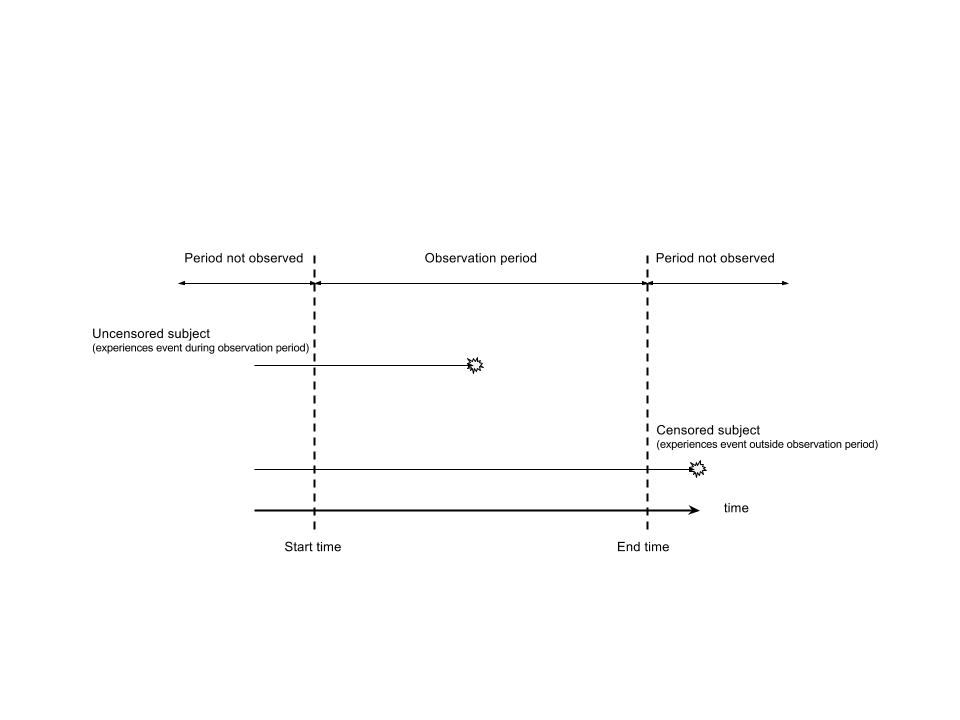
\includegraphics[width=\textwidth]{Data_censoring.png}
        \caption{Censored and uncensored data}
        \label{img:data_censoring}
      \end{figure}

      There are different situations of data censoring, right, left and interval censoring. \emph{Right censoring} refers to the situation when the event doesn't occur during the observation period and occurs time after the end of the observation time interval. On the other hand, \emph{left censoring} occurs when the subjects of the study have already experienced the event when the study starts, but it is not clear exactly when. \emph{Interval censoring} refers to the case when the event has occurred during the interval but the information about the time it happened is not available.

      Truncation is when there is a period of time when there is no information, inside the observation period. There are also three different types of truncations, right and left truncation, and interval truncation, being the most usual left or interval truncation, and the rarest right truncation.

    \subsection{Data structure}

      As commented before, there is a specific format for the data input in the survival analysis models, this format is briefly explained below.

      There are three main structures of data input: single-episode or subject-based, multi-episode based and person or subject-period files, also called discrete-time data files.

      \subsubsection{Single-episode data}

        In single-episode structured files, each row corresponds to a different subject, and the columns represent the variables and the events occurred. It implies that if a subject experiments more than one event, it is registered on the same row, as there ir no information of the instance on any other row.

      \subsubsection{Multi-episode data}

        Multi-episode file represents a subjects that experiment the event more than one time, and the data from each subject is separated in different rows for each event, where the first event is in the first row of the instance and the subsequent events, in case there are, are represented on the consecutive rows, having each subject as much rows as events the subject experiences.

  \section{Kaplan-Meier Estimator model}

    Most survival analysis studies start with a non-parametric method as they are simple and fast, and provide with an intuitive graphical form of understanding the data. The two main non-parametric methods, as mentioned before are the Life Tables and the Kaplan-Meier Estimator model. The first is more adequated for large datasets and when the time is not measured with precision. On the other hand, the KM Estimates method is great for when the time is precisely measured, and is widely used, more than the life tables.

    The main idea of the KM method is to estimate the survival function at a time 't' $\widehat{S}(t)$, which is the probability of a subject surviving until this time 't'. It can be calculated by obtaining the conditional probability of not experiencing the event on time 't', not having experienced it in previous failure times:

    \begin{equation}
      \widehat{S}(t_{(j)}) = \widehat{S}(t_{(j-1)}) \times Pr(T>t_{(j)}|T \geq t_{(j)})
      % \caption{Survival function at time t$_j$ in terms of the previous survival interval and probabilities for the KM Estimates model}
      \label{eq:KM-eq-surv}
    \end{equation}

    The previous equation can also be written as follows, in terms of conditional probability for a specific time:

    \begin{equation}
      \widehat{S}(t_{(j)}) = \prod_{i=1}^{j-1} Pr(T>t_{(i)}|T\geq t_{(i)})
      % \caption{Survival function at time t$_j$ in terms of probabilities for the KM Estimates model}
      \label{eq:KM-eq-probab}
    \end{equation}

    The KM model is a non-parametric, maximum likelihood model, which means that it relies on the maximization of the likelihood function of the sample to analyze. This likelihood function takes the following form:

    \begin{equation}
      L = \prod_{i=1}^k h_i^{d_i}(1-h_i)^{n_i-d_i}
      % \caption{Likelihood function for the KM Estimates model}
      \label{eq:km-likelihood-function}
    \end{equation}

    where \emph{n$_i$} represents the number of individuals at risk at a certain time, and \emph{d$_i$} represents the number of events occurred at this particular time. Maximizing this function, the hazard function can be obtained in terms of \emph{n$_i$} and \emph{d$_i$} for each time:

    \begin{equation}
      \widehat{h_i}=\frac{d_i}{n_i}, \ for \ i = 1,2,...,k
      % \caption{Hazard function for the KM Estimates model}
      \label{eq:km-hazard-function}
    \end{equation}

    and the survival function for each time has the following form:
    \begin{equation}
      \widehat{S(t_i)} = \prod_{i | t_i < t_k}(1 - \frac{d_i}{n_i})
      % \caption{Survival function in terms of the number of events in a time period and the number of surviving elements at this time for the KM Estimates model}
      \label{eq:km-survival-function}
    \end{equation}

    Assuming asymptotic result, for big series of data in the sample, the variance of the maximum likelihood estimator can be obtained:

    \begin{equation}
      \widehat{Var} = \frac{d_i(d_i-n_i}{n_i^3}
      \label{eq:km-havar-variance}
    \end{equation}

    and with this an estimation of the variance of the survival function, resulting in the \emph{Greenwood equation}:

    \begin{equation}
      \widehat{Var}(\widehat{S}(t_i)) = \widehat{S}(t_i)^2 \sum_{j=1}^{i-1} \frac{d_j}{d_j(n_j-d_j)}
      \label{eq:km-greenwood-eq}
    \end{equation}

    Considering the asymptotic convergence to normal distribution of the maximum likelihood estimators, confidence intervals for $(1 - a)\%$ can be calculated for this estimations:

    \begin{equation}
      \widehat{S}(t_i)\pm Z_{a/2}\sqrt{\widehat{Var}(\widehat{S}(t_i))}
      \label{eq:km-confidence-intervals}
    \end{equation}

    One interesting advantage of the Kaplan-Meier Estimates model is the visualization of the survival function in a graph, as this method is intended for exploratory analysis and for a light approach to the problem itself, the possibility of plotting the results in a easy to understand graph is an interesting feature. In comparison with other algorithms outside survival analysis, the main advantage is the ability to account for the censored data.

    The other side of the simplicity of the model is that it only provides probability estimations on the whole group, it does not take account of other explanatory variables. This limitation constraints the analysis to homogeneous groups, where the other explanatory variables are homogeneous along all the sample. To mitigate this limitation when the sample is not homogeneous on the other explanatory variables, it can be separated in more homogeneous groups and apply the method to each group, being able to compare the results of every subsample.


  \section{Cox Proportional Hazards Model}

    Cox Proportional Hazards Model is one of the most relevant regarding time series in general and survival analysis in particular. The model was introduced in 1972 by Sir David Cox in the paper \emph{Regression models and life tables}, and introduced two key features, in first place, the proportional hazards model, in second place the method of partial likelihood estimation.

    The


    The Cox Proportional Hazards model can be used both for time-fixed or time-varying covariates.

    \subsection{Cox Proportional Hazards Model for time-fixed covariates}

      Time-fixed covariates are the ones that remain constant on the whole study, and are characteristics of the subjects, for example the gender or the place of birth. The expression of the hazard function for each individual ($i$) at time ($t$) in the basic time-fixed for covariates model is the following:

      \begin{equation}
        h_i(t) = h_0(t)\exp(\beta_1x_{i1} + \beta_2x_{i2} + \cdots + \beta_kx_{ik})
        \label{eq:cox-fixed-time-hazards}
      \end{equation}

      where the $x_{ik}$ represent the values of each covariate ($k$) for each individual of the sample, $h_0$ is the \emph{baseline hazard function}, which represents the hazard that does not depend on the individual, common for everyone. The intercept of the function is contained on this baseline hazard function.

      The equation can be written in terms of \emph{log hazard ratio}:

      \begin{equation}
        \log\left(\frac{h_i(t)}{h_0(t)}\right) = \beta_1x_{i1} + \cdots + \beta_kx_{ik}
        \label{eq:cox-fixed-time-log-hazards-rate}
      \end{equation}

      this

    \subsection{Cox Proportional Hazards Model for time-varying covariates}
















  \subsection{SystemML input \& output format}

    As described on the oficial documentation of Apache SystemML, to run a survival analysis using the KM estimates method or Cox Proportional Hazards model, three files have to be provided, containing three matrixes, the data itself in the appropriate format, along with two other matrix indicating position of specific variables inside the former. These files are specified on each algorithm's description, as the project is open source, the algorithm implementation can be seen on the project's Github page \cite{systemml_github_page}.

    Apart from the files specified on the oficial documentation and the algorithm implementation, it is also necessary to provide, along with every matrix file, another file with the same name, and the \emph{.mtd} extension, containing the information of the file containing the matrix in JSON format:

    \begin{lstlisting}[label=matrix_metadata_file, language=sh, caption=Example of matrix metadata file in JSON format]
      {
        "data_type": "matrix",
        "value_type": "double",
        "rows": 10,
        "cols": 3,
        "nnz": 10,
        "format": "csv",
        "header": false,
        "sep": ",",
        "description": {
            "author": "SystemML"
        }
      }
    \end{lstlisting}

\newpage

    \subsubsection{Kaplan Meier Estimates}

      According to the oficial documentation, the files and parameters needed to execute the KM Estimates algorithm are the following:

      \begin{table}[!ht]
        \centering
        \begin{tabular}{|>{\centering\arraybackslash}m{0.2\textwidth}|m{0.8\textwidth}|}
          \hline
            \thead{File} \thead{or parameter} & \thead{Content or value} \\
            \bottomrule
            X & input matrix with the survival data itself, containing the following variables, separated in columns: timestamps, whether the event occurred $(1)$ or the data is censored $(0)$, columns with categorical features for grouping and/or stratifying \\ \hline
            TE & input column matrix indicating the indices of the columns where the timestamps and the event information are located on matrix \emph{X} \\ \hline
            GI & input column matrix indicating the indices of the columns where the categorical values used for grouping are stored on matrix \emph{X} \\ \hline
            SI & input column matrix indicating the indices of the columns where the categorical values used for stratifying are stored on matrix \emph{X} \\ \hline
            F & input column matrix  indicating the indices of X which are to be used for KM analysis \\ \hline
            alpha & parameter to compute confidence intervals for the survivor function and its median \\ \hline
            etype & parameter to specify the error type, \emph{greenwood} or \emph{peto} \\ \hline
            ctype & parameter to modify the confidence interval, \emph{plain} remains the lower and upper bound of the confidence interval unmodified, \emph{log} corresponds to the logistic transformation, and \emph{log-log} corresponds to the complementary log-log transformation \\ \hline
            ttype & if data from different groups is available, parameter to specify the test to perform for comparing survival data across multiple groups, the options are: \emph{none}, \emph{log-rank} and \emph{wilcoxon} \\ \hline
            fmt & parameter to specify the output format to use for the results: \emph{text} or \emph{csv} \\ \hline
        \end{tabular}
        \caption{Input files and parameters for Kaplan-Meier Estimates algorithm}
        \label{tab:KM_IO_files}
      \end{table}

\newpage

      \begin{table}[!ht]
        \centering
        \resizebox{\textwidth}{!}{
        \begin{tabular}{|>{\centering\arraybackslash}m{0.2\textwidth}|m{0.8\textwidth}|}
          \hline
            \thead{File} \thead{or parameter} & \thead{Content or value} \\
            \bottomrule
            O & output matrix containing the results of the Kaplan-Meier analysis, with $7$ columns that represent the status on each time interval:
            \begin{itemize}
              \item timestamp
              \item number of subjects at risk
              \item number of events
              \item KM estimate of the survival function
              \item Standard error of survival function
              \item Lower confidence interval for survival function
              \item Upper confidence interval for survival function
            \end{itemize} \\ \hline
            M & output matrix whose dimension depends on the number of groups (g) and strata (s) in the data (k denotes the number of factors used for grouping, i.e., ncol(GI) and l denotes the number of factors used for stratifying, i.e., ncol(SI)):
            \begin{itemize}
              \item unique combination of values in the k factors used for grouping
              \item unique combination of values in the l factors used for stratifying
              \item total number of records
              \item total number of events
              \item median
              \item lower $100*(1-alpha)\%$ confidence interval of the median of survival function
              \item upper $100*(1-alpha)\%$ confidence interval of the median of survival function
            \end{itemize} \\ \hline
            T & if survival data from multiple groups is available, and \emph{ttype} is \emph{log-rank} or \emph{wilcoxon}, output matrix containing the result of the stratified test for comparing multiple groups:
            \begin{itemize}
              \item number of groups
              \item degree of freedom for Chi-squared distributed test statistic
              \item test statistic
              \item p-value
            \end{itemize}
             \\ \hline
            T\_GROUPS\_OE & if exists T, statistics for groups formed on analysis, with as many rows as groups, and the following column values:
            \begin{itemize}
              \item number of events
              \item observed value
              \item expected value
              \item $(O-E)^2/E$
              \item $(O-E)^2/V$
            \end{itemize}
            \\ \hline
        \end{tabular}}
        \caption{Output files and parameters for Kaplan-Meier Estimates algorithm}
        \label{tab:KM_IO_files}
      \end{table}

      \begin{minipage}[b][7.7cm][b]{0.35\textwidth}

        \begin{lstlisting}[label=km_input_matrix, language=sh, caption=Input X matrix for KM Estimates model]
          0,0,1.0
          0,0,1.0
          0,0,1.0
          0,0,1.0
          0,0,1.0
          0,0,1.0
          0,0,1.0
          0,0,1.0
          0,0,1.0
          0,0,1.0
        \end{lstlisting}

      \end{minipage}
      \begin{minipage}[b][7.7cm][b]{0.6\textwidth}

        \begin{lstlisting}[label=km_input_matrix_meta, language=sh, caption=Input X metadata matrix for KM Estimates model]
          {
            "data_type": "matrix",
            "value_type": "double",
            "rows": 10,
            "cols": 3,
            "nnz": 10,
            "format": "csv",
            "header": false,
            "sep": ",",
            "description": {
                "author": "SystemML"
            }
          }
        \end{lstlisting}

      \end{minipage}

      This sample files can be generated via script located in the github repository, on the scripts directory. It is recommendable to do so, to see the appropriate input format the files have for the algorithm, an example of the invocation of this sample generation script is shown below\footnote{More information about the parameters and configuration to run the data generation can be found on the script itself, available on the SystemML github repository.}:

      \begin{lstlisting}[label=data-generation-invocation, language=sh, caption=Sample invocation of the data generation script]
        #!/bin/bash
        <SPARK_HOME>/bin/spark-submit <systemml-path>/SystemML.jar\
        -f <systemml-scripts-path>/datagen/genRandData4SurvAnalysis.dml\
        -nvargs type=kaplan-meier\
        n=<number-samples>\
        p=<probability-of-not-censoring>\
        O=<O-file-path>\
        TE=<TE-file-path>\
        fmt=<format>
        g=<groups>
        s=<strata>
        f=<number-of-levels-for-cathegorical>
      \end{lstlisting}

\newpage

    \subsubsection{Cox Proportional Hazards Model}

      The Cox Proportional Hazards model is, as seen above, quite different from the KM estimates, and needs the following files and parameters:

      \begin{table}[!h]
        \centering
        \begin{tabular}{|>{\centering\arraybackslash}m{0.2\textwidth}|m{0.8\textwidth}|}
          \hline
            \thead{File} \thead{or parameter} & \thead{Content or value} \\
            \bottomrule
            X & input matrix with the survival data itself, containing the following variables separated in columns: timestamps, whether the event occurred (1) or the data is censored (0), columns of features for the model \\ \hline
            TE & input matrix indicating the indexes of the columns where the timestamps and the event information are located on matrix X \\ \hline
            F & input column matrix  indicating the indices of X which are to be used for fitting the Cox model \\ \hline
            R & If factors (categorical variables) are available in the input matrix X, matrix containing the start and end indices of the factors in X
              \begin{itemize}
                \item R[,1]: start indices
                \item R[,2]: end indices
              \end{itemize}

								Alternatively, user can specify the indices of the baseline level of each factor which needs to be removed from X.

                If R is not provided by default all variables are considered to be continuous \\ \hline
            alpha & parameter to compute confidence intervals, $100*(1 - alpha)\%$ for the betas of the model \\ \hline
            tol & tolerance, $\epsilon$ \\ \hline
            moi & maximum number of outer iterations, using Newton method \\ \hline
            mii & maximum number of inner iterations, using conjugate gradient method, if this value is $0$, there will be no maximum \\ \hline
            fmt & format of the output matrixes, it can be csv or txt \\ \hline
        \end{tabular}
        \caption{Input files and parameters for Cox Proportional Hazards algorithm}
        \label{tab:Cox_IO_files}
      \end{table}

\newpage

      \begin{table}[!h]
        \centering
        \begin{tabular}{|>{\centering\arraybackslash}m{0.2\textwidth}|m{0.8\textwidth}|}
          \hline
            \thead{File} \thead{or parameter} & \thead{Content or value} \\
            \bottomrule
            M & output matrix with dimensions $D \times 7$, where D is the number of covariates of the model, and the columns represent:
            \begin{itemize}
              \item betas $(\beta_i)$
              \item $exp(\beta_i)$
              \item standard error of $\beta_i$
              \item Z
              \item p-value
              \item lower $100*(1-alpha)\%$ confidence interval of $\beta_i$
              \item upper $100*(1-alpha)\%$ confidence interval of $\beta_i$
            \end{itemize}
            \\ \hline
            S & output log file containing a summary of statistics of the model:
            \begin{itemize}
              \item number of observations
              \item number of events
              \item log-likelihood
              \item AIC
              \item Rsquare (Cox \& Snell)
              \item max posible Rsquare
            \end{itemize}
            \\ \hline
            T & output log file containing a summary of statistics of the model, with the following format in lines:
            \begin{itemize}
              \item Likelihood ratio test statistic, degree of freedom, P-value
              \item Wald test statistic, degree of freedom, P-value
              \item Score (log-rank) test statistic, degree of freedom, P-value
            \end{itemize}
            \\ \hline
            RT & output column matrix containing the order-preserving recorded timestamps from X \\ \hline
            XO & output matrix, which is the same of X but with timestamps \\ \hline
            COV & output matrix containing the variance-covariance matrix of betas \\ \hline
            MF & output column matrix containing the column indices of X with the baseline factors removed (if available) \\ \hline
        \end{tabular}
        \caption{Output files and parameters for Cox Proportional Hazards algorithm}
        \label{tab:Cox_IO_files}
      \end{table}

\newpage

  \section{Algorithm invocation}

    The algorithm scripts have a sample invocation of them to be executed in a Hadoop environment, the execution over Spark is similar:

    \begin{lstlisting}[label=code:km-invocation-spark, language=sh, caption=Example of the invocation of the Kaplan-Meier Estimates model with Apache SystemML over an Apache Spark framework]
    #!/bin/bash
    <SPARK_HOME>/bin/spark-submit <path-to-systemml>/SystemML.jar\
    -f <path-to-systemml-algorithms>/scripts/algorithms/KM.dml\
    -nvargs X=<file-X-location>\
            TE=<file-TE-location>\
            GI=<file-GI-location>\
            SI=<file-SI-location>\
            O=<file-O-location>\
            M=<file-M-location>\
            T=<file-T-location>\
            alpha=<alpha>\
            etype=<error-type>\
            ctype=<confidence-interval-tunning>\
            ttype=<test-type>\
            fmt=<output-format>
    \end{lstlisting}

    \begin{lstlisting}[label=code:km-invocation-spark, language=sh, caption=Example of the invocation of the Cox Proportional Hazard model with Apache SystemML over an Apache Spark framework]
    #!/bin/bash
    <SPARK_HOME>/bin/spark-submit <path-to-systemml>/SystemML.jar\
    -f <path-to-systemml-algorithms>/scripts/algorithms/Cox.dml\
    -nvargs X=<file-X-location>\
    TE=<file-TE-location>\
    F=<file-F-location>\
    R=<file-R-location>\
    M=<file-M-location>\
    S=<file-S-location>\
    T=<file-T-location>\
    COV=<file-COV-location>\
    RT=<file-RT-location>\
    XO=<file-XO-location>\
    MF=<file-MF-location>\
    alpha=<alpha>\
    tol=<tolerance-epsilon>\
    moi=<max-outer-iterations>\
    mii=<max-inner-iterations>\
    fmt=<output-format>
    \end{lstlisting}

    Note that the input and output matrixes are files, and the algorithms have to have the path to them as input arguments, they also need the parameters set on the invocation of the algorithm, otherwise, default values will be used. It is also important to note that, as commented before, along with the file containing the matrix, another file containing the metadata associated to the matrix have to be provided, as can be seen on the code examples of \ref{km_input_matrix} and \ref{km_input_matrix_meta}.

    As the execution of the algorithm is a jar file given to spark-submit, all the spark's configuration can be set, thus the execution on a distributed environment would be almost the same, but with the specific Spark's configuration to run in distributed mode with the desired resources and security configuration.

    The execution can also be done in the Jupyter Notebook, as the algorithm's script is open source, just copying the code into a cell and calling the function with the desired parameters.


\chapter{Conclusions}
  \label{sec:conclusions}

  \section{Most important results}

  \section{Lessons learnt}

\newpage


\nocite{*}
\newpage
\printbibliography

\end{document}
